
\documentclass{article}
\usepackage{amssymb}
\usepackage{amsmath}
\usepackage{graphicx}
\usepackage{subfigure}
\begin{document}

\section{2D Random Walk}
To solve this problem, we first obtain $x_{n}$ for one random walker. Put a
random walker at the origin. Create a random number $movestep$ in range
(0,1,2,3), and these four numbers means moving one step right/left/up/down
respectively. We use a list to record the number of moving steps in every
direction. After we get the moving direction of a step, we add the number of
total steps in that certain direction by 1. If the total number of moving
steps is $n$, we repeat the previous procedure $n$ times. The number of
total rightward steps minus the number of total leftward steps generates the
x-component of the random walker's displacement, $x_{n}$. Likewise, the
number of total upward steps minus the number of total downward steps
generates the y-component of the random walker's displacement, $y_{n}$. 
After that, $x_{n}^{2}$ and $r_{n}^{2}$ are easy to calculate. We use a
function named random\_walk to return the values of $x_{n}$,  $x_{n}^{2}$,
and $r_{n}^{2}$. Since our goal is averaging over $10^{4}$ different
walkers, we need a loop with $10^{4}$ iterations to get the values of $%
x_{n}$, $x_{n}^{2}$, and $r_{n}^{2}$ of each walker, and then realize the
average values, $\left\langle x_{n}\right\rangle $, $\left\langle
x_{n}^{2}\right\rangle $, and $\left\langle r_{n}^{2}\right\rangle $. 
\begin{figure}[!ht]
	\centering
	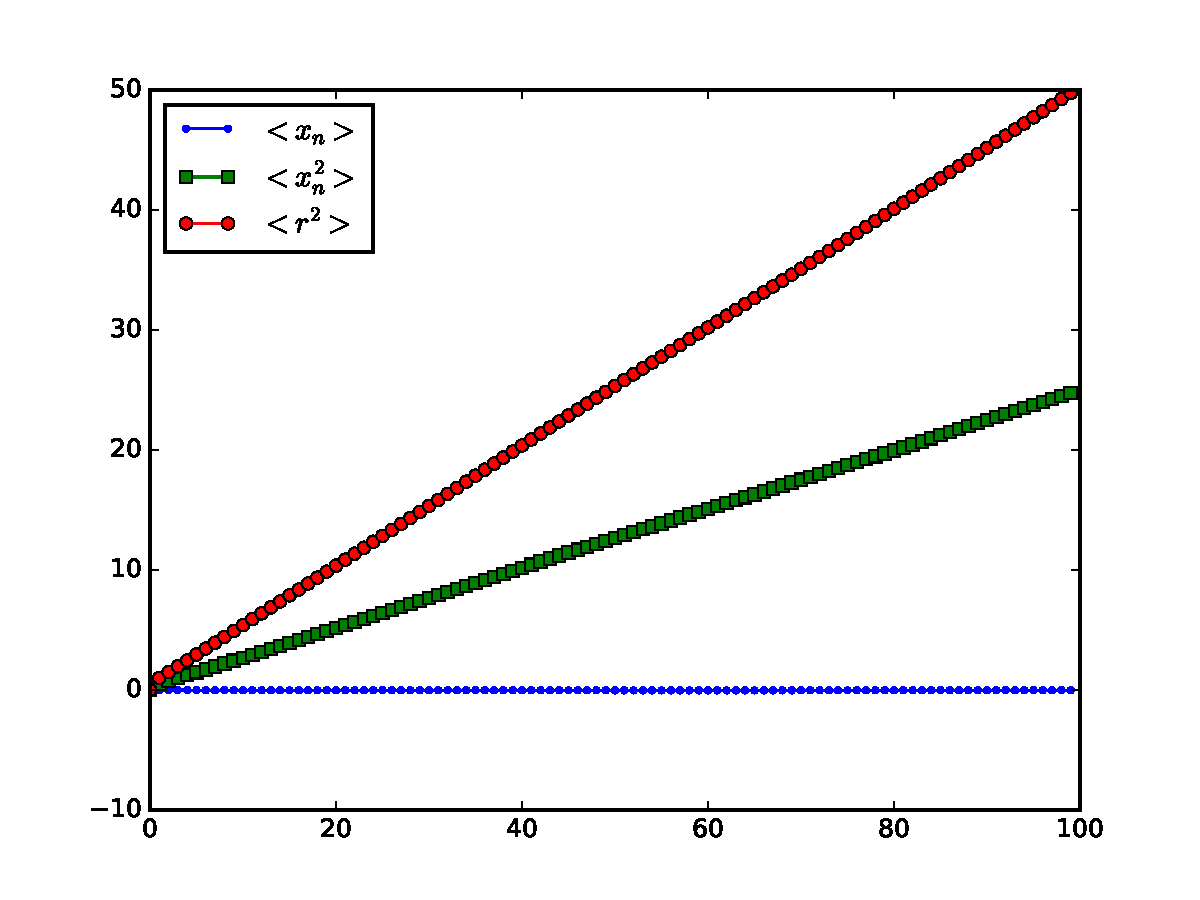
\includegraphics[width=0.82\textwidth, clip]{RandomWalk.pdf}
	\caption{}
\end{figure}

\end{document}
